    \documentclass{article}
    \usepackage{fancyhdr, amsmath, amsthm, amssymb, mathtools, lastpage, hyperref, enumerate, graphicx, setspace, upgreek}
    \usepackage[margin=1in, top=0.8in,bottom=0.8in]{geometry}
    \usepackage{subcaption}
	\renewcommand{\thesubsection}{\alph{subsection})}
    \newcommand{\scinot}[2]{#1\times10^{#2}}
    \newcommand{\bra}[1]{\left<#1\right|}
    \newcommand{\ket}[1]{\left|#1\right>}
    \newcommand{\dotp}[2]{\left<#1\,\middle|\,#2\right>}
    \newcommand{\rd}[2]{\frac{\mathrm{d}#1}{\mathrm{d}#2}}
    \newcommand{\pd}[2]{\frac{\partial#1}{\partial#2}}
    \newcommand{\rtd}[2]{\frac{\mathrm{d}^2#1}{\mathrm{d}#2^2}}
    \newcommand{\ptd}[2]{\frac{\partial^2 #1}{\partial#2^2}}
    \newcommand{\norm}[1]{\left|\left|#1\right|\right|}
    \newcommand{\abs}[1]{\left|#1\right|}
    \newcommand{\pvec}[1]{\vec{#1}^{\,\prime}}
    \newcommand{\tensor}[1]{\overleftrightarrow{#1}}
    \let\Re\undefined
    \let\Im\undefined
    \newcommand{\ang}[0]{\text{\AA}}
    \newcommand{\mum}[0]{\upmu \mathrm{m}}
    \DeclareMathOperator{\Re}{Re}
    \DeclareMathOperator{\Tr}{Tr}
    \DeclareMathOperator{\Im}{Im}
    \DeclareMathOperator{\E}{E}
    \DeclareMathOperator{\Var}{Var}
    \newcommand{\expvalue}[1]{\left<#1\right>}
    \usepackage[labelfont=bf, font=scriptsize]{caption}\usepackage{tikz}
    \usepackage[font=scriptsize]{subcaption}
    \everymath{\displaystyle}

\begin{document}
\title{Ph20.1 - Introduction to Python\\ Lissajous figures and Beats}
\author{Cassidy Yang}
\maketitle
\pagestyle{fancy}
\rhead{Cassidy Yang}
\cfoot{Page \thepage \hspace{1pt} of \pageref{LastPage}}

\section{The Assignment}

The corresponding Python code is attached in a separate document.

\begin{enumerate}
	\item Lissajous figures.
	
	The Y vs. X plots are closed curves for which $\frac{f_x}{f_y}$ are rational numbers. The following figure includes the graphs for which the ration $\frac{f_x}{f_y}$ is equal to $\frac{1}{2}, \frac{2}{3}, 1$, and 2 (see Figure 1). We note that upon initial inspection, it seems that Figures 1b, c seem to be open curves. However, in actuality, the curve retraces itself to form a closed curve.
	
	\begin{figure}[h]
		\centering
		\begin{subfigure}{0.4\textwidth}
		\centering
		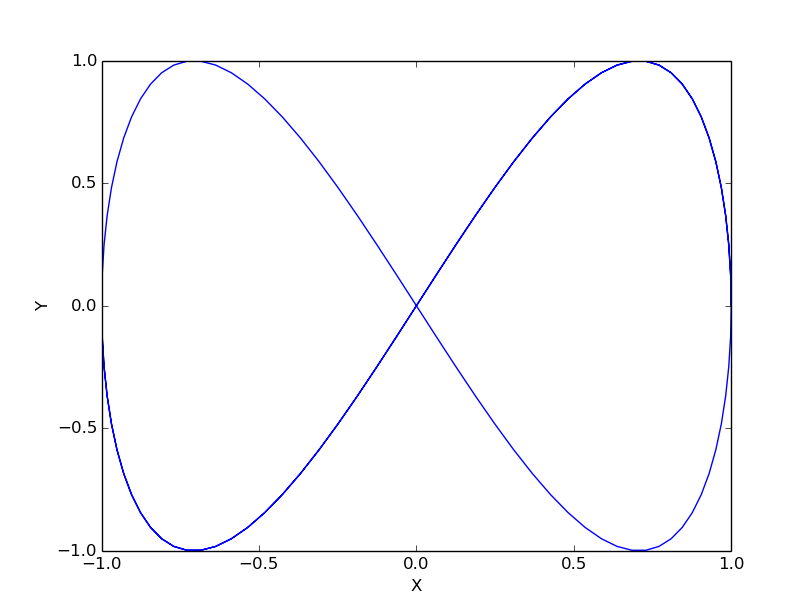
\includegraphics[width=0.9\linewidth]{fig1.png}
		\caption{$\frac{f_x}{f_y} = \frac{1}{2}$}
		\end{subfigure}
		~
		\begin{subfigure}{0.4\textwidth}
		\centering
		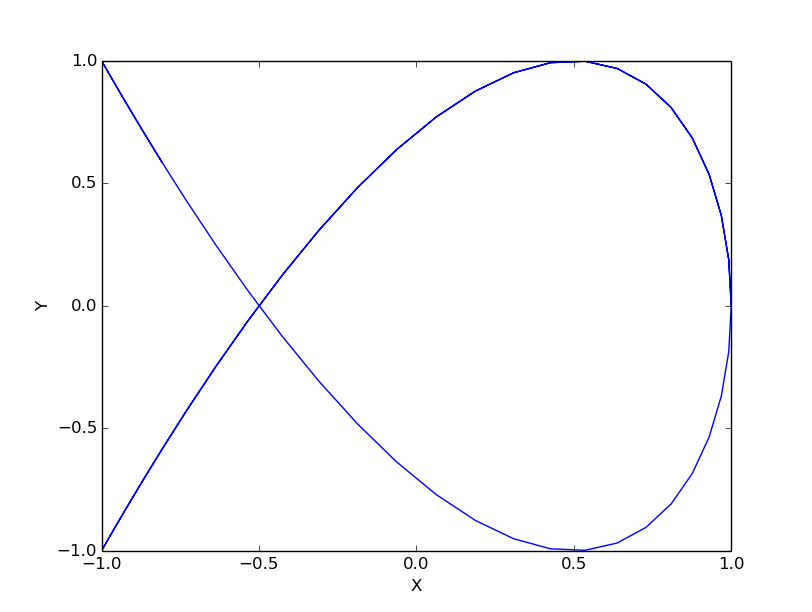
\includegraphics[width=0.9\linewidth]{fig2.png}
		\caption{$\frac{f_x}{f_y} = \frac{2}{3}$}
		\end{subfigure}
		
		\begin{subfigure}{0.4\textwidth}
		\centering
		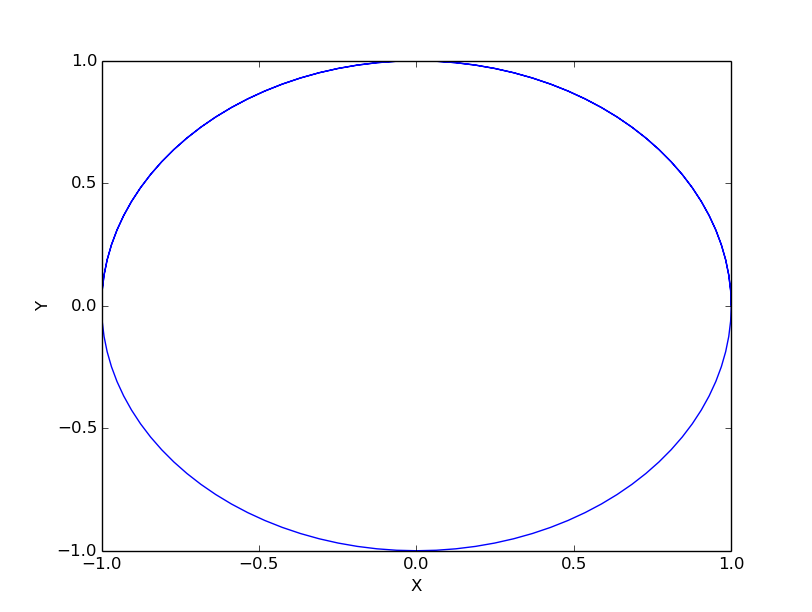
\includegraphics[width=0.9\linewidth]{fig3.png}
		\caption{$\frac{f_x}{f_y} = 1$}
		\end{subfigure}
		~
		\begin{subfigure}{0.4\textwidth}
		\centering
		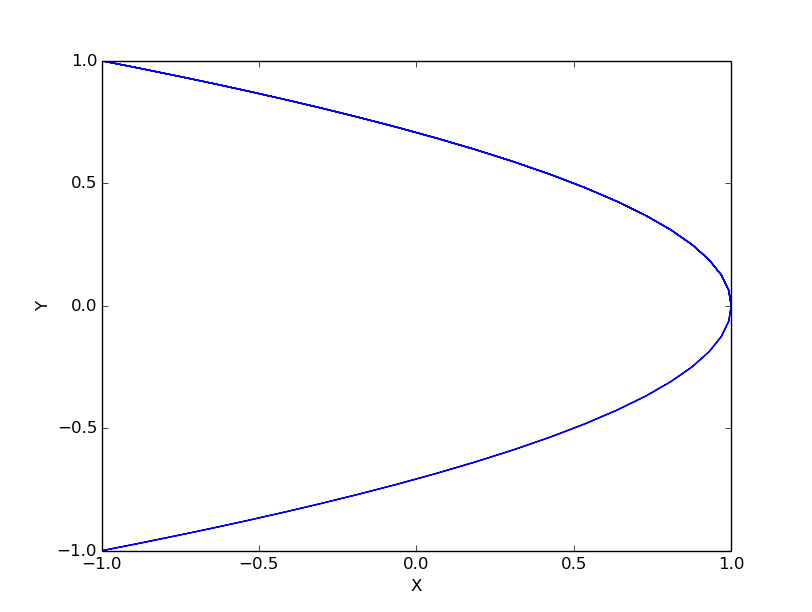
\includegraphics[width=0.9\linewidth]{fig4.png}
		\caption{$\frac{f_x}{f_y} = 2$}
		\end{subfigure}
		
		\caption{Y vs. X plots for various ratios of $\frac{f_x}{f_y}$}
		
	\end{figure}
	
	We note that the as $\frac{f_x}{f_y}$ diverges from 1, more loops are added to the graph. We can see this by comparing the graphs below, in which $\frac{f_x}{f_y} = \frac{1}{5}$ (Figure 2a) and 1 (Figure 2b). Furthermore, as the ratio gets larger, more wavelengths are formed in the y direction, and as the ratio gets smaller, more wavelengths are formed in the x direction.
	
	\begin{figure}[h]
		\centering
		\begin{subfigure}{0.4\textwidth}
		\centering
		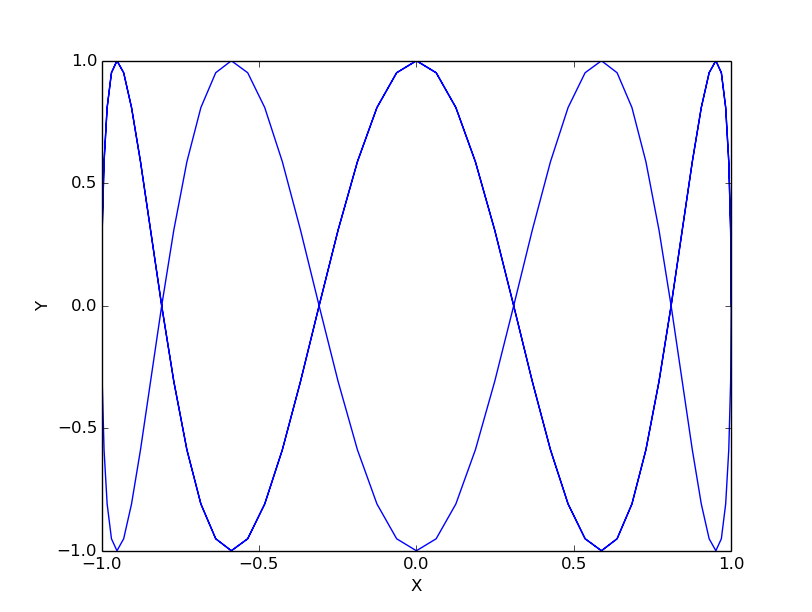
\includegraphics[width=0.9\linewidth]{fig5.png}
		\caption{$\frac{f_x}{f_y} = \frac{1}{5}$}
		\end{subfigure}
		~
		\begin{subfigure}{0.4\textwidth}
		\centering
		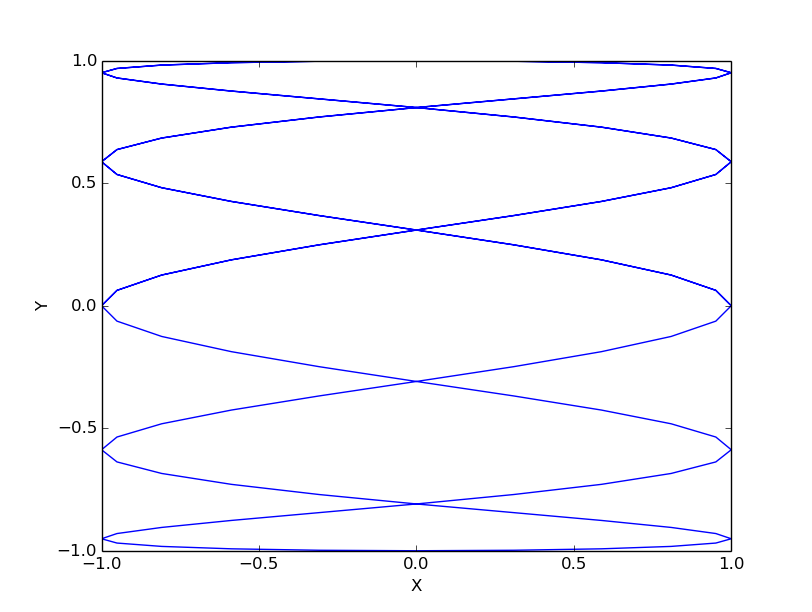
\includegraphics[width=0.9\linewidth]{fig6.png}
		\caption{$\frac{f_x}{f_y} = 5$}
		\end{subfigure}
		
		\caption{Investigation of $\frac{f_x}{f_y}$ ratio}
	\end{figure}
	
	Now for the case $f_X = f_Y$, let us examine the changes to the shape of the curve at various phase shifts. The following figure are Y vs. X graphs with phase shifts $\phi = -0.314, 0, 0.314, 0.8$. For positive phase shifts, the circle narrows along the $y = x$ line as the magnitude of the phase shift increases. For negative phase shifts, the circle narrows along the $y = -x + 1$ line as the magnitude of the phase shift increases. 
	
	\begin{figure}[h]
		\centering
		\begin{subfigure}{0.4\textwidth}
		\centering
		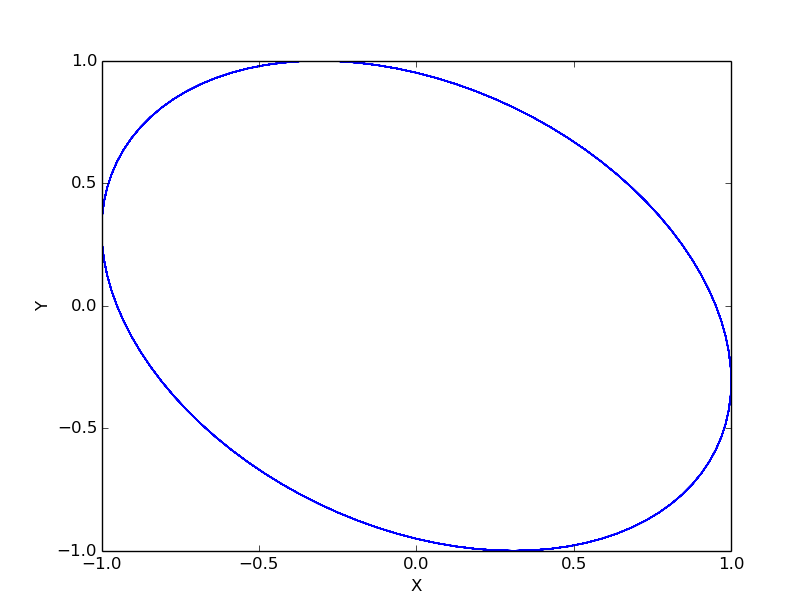
\includegraphics[width=0.9\linewidth]{fig8.png}
		\caption{$\phi = -0.314$}
		\end{subfigure}
		~
		\begin{subfigure}{0.4\textwidth}
		\centering
		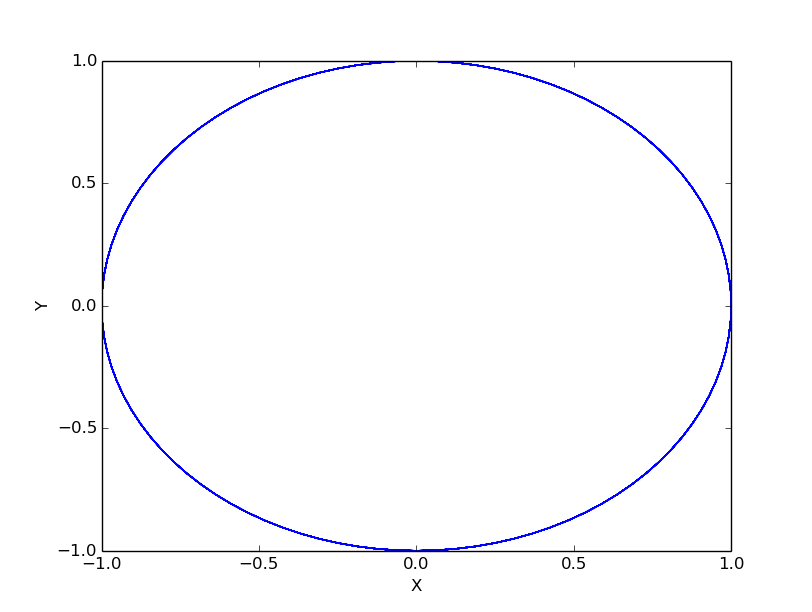
\includegraphics[width=0.9\linewidth]{fig9.png}
		\caption{$\phi = 0$}
		\end{subfigure}
		
		\begin{subfigure}{0.4\textwidth}
		\centering
		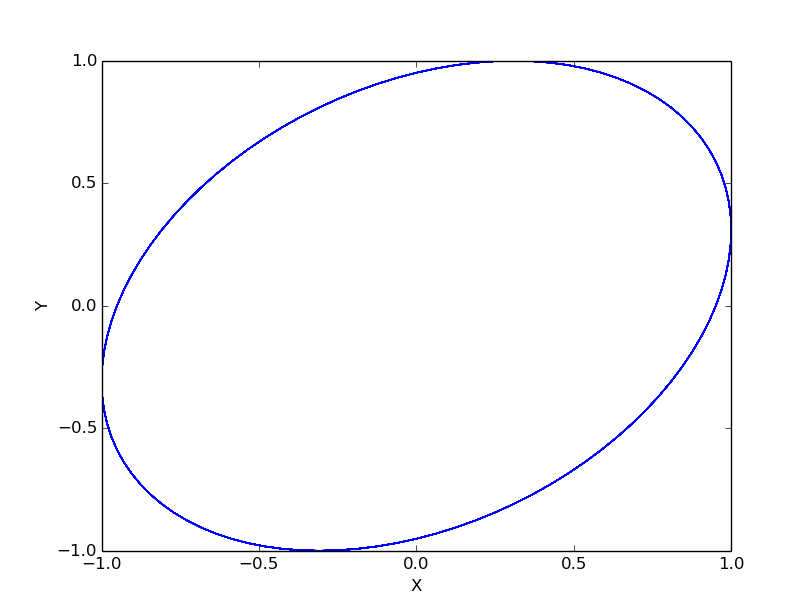
\includegraphics[width=0.9\linewidth]{fig10.png}
		\caption{$\phi = 0.314$}
		\end{subfigure}
		~
		\begin{subfigure}{0.4\textwidth}
		\centering
		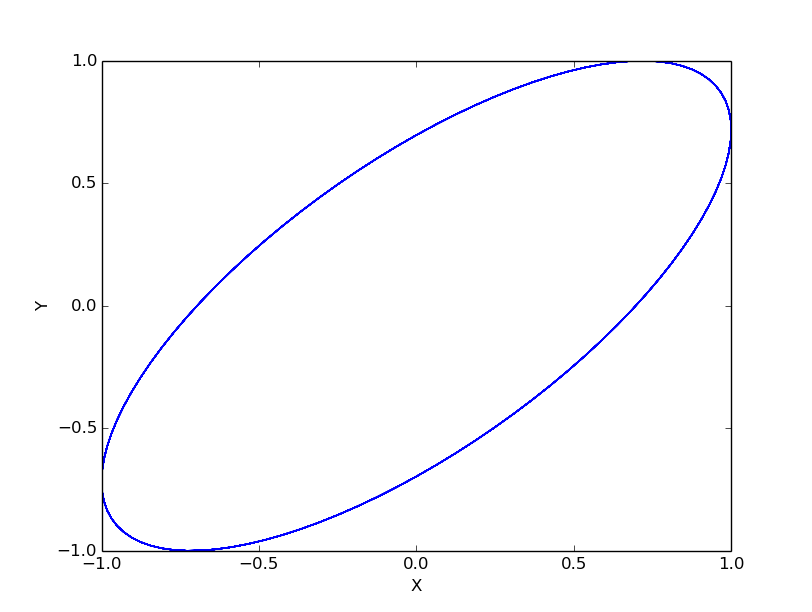
\includegraphics[width=0.9\linewidth]{fig11.png}
		\caption{$\phi = 0.8$}
		\end{subfigure}
		
		\caption{Investigation of phase shift $\phi$}
		
	\end{figure}
	
	We can take advantage of this fact to tune electronic circuits. If we connect two different sinusoidal inputs into the two channels of an oscilliscope (which would be able to produce the Y vs. X graphs of the inputs), we will be able to detect the phase difference between the two different inputs. The two frequencies can then be tuned until we see a symmetric curve (Figure 3b), which is indicative of no phase difference.

	\item Beats.
	
	In order to examine the beats phenomenon, we set $f_X = 1$ and $f_Y = 1.1$. The corresponding $Z(t)$ plot as a function of $t$ is shown in Figure 4.
	
	\begin{figure}[h]
		\centering
		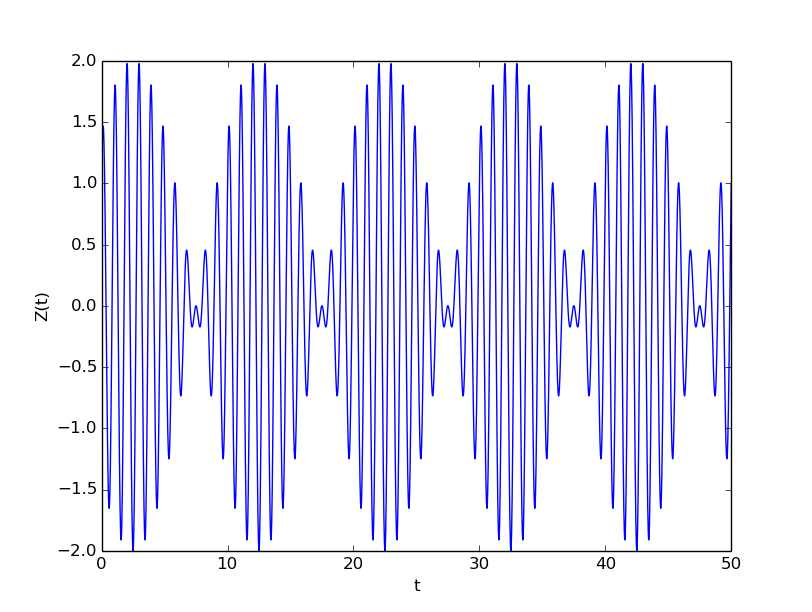
\includegraphics[width=0.4\linewidth]{fig12.png}
		
		\caption{Beats phenomenon for $f_X = 1$ $f_Y = 1.1$}
	\end{figure}
	
	We note that in this case, the carrier frequency is $\frac{\omega_1 + \omega_2}{2} = (f_x + f_y) \pi = 2.1 \pi$. The modulation cycles have frequency of $(\omega_1 - \omega_2) = (f_x - f_y)(2\pi) = 0.2\pi$. Note that the modulation frequency is about twice the expected ($(\omega_1 - \omega_2)$ vs. $\frac{(\omega_1 - \omega_2)}{2}$), since cosine is an even function and the modulation for positive and negative values have the same resultant wave form. The two halves of the envelope are identical, so the modulation frequency is $0.2\pi$.
	
	\item This week's experience.
	
	This week, I spent some time getting up to speed with using Unix, which I wasn't (and still am not) too comfortable with. I decided to dual-boot my system in hopes to have more practice with it and learn it better. I am still getting used to the system and learning new commands.
	
	Additionally, I had to relearn some of Python, since I had not used it for a while. However, relearning python did not take too long, since the first lab did not require complicated code. I was able to pick it up by simple google searches and looking at some example code. I do agree with Guido van Rossum; picking up (and repicking up) Python is fairly easy, especially since it contains so much syntatic sugar. The straightforward syntax also makes debugging fairly easy to implement.

\end{enumerate}



\end{document}